\section{The average drag force correlation}
\label{sec:model_drag}
In this section, we start by reviewing the various existing models for the averaged drag force acting on fluid inclusions in the Stokes regime. 
Subsequently, we consider the intermediate Reynolds number regime. 
The primary focus of our current investigation, is to propose a drag model that reasonably fits the numerical results. 
As demonstrated in the previous section, the droplet maintains an approximate spherical shape within the range of parameters studied here. 
Although slight deviations from sphericity are noted for $Bo=0.5$ and in configurations with the highest inertia, the maximum deviation from the spherical shape remains moderate less than $5$ \%. 
Hence, in this section we assume that fluid inclusions are spherical.



\subsection{Stokes flow regime}

From an experimental standpoint, quantifying the force exerted on ascending fluid particles in moderately dense conditions and establishing its correlation with the kinematic properties of both the fluid and the particles poses considerable challenges. 
Nonetheless, a feasible alternative involves measuring the mean settling or rising velocity of a suspension by measuring the velocity of its front \citep{guazzelli2011}. 
In a confined vessel, the mean velocity of fluid particles undergoing settling or rising is known to be hindered; that is, it decreases in comparison to the velocity of an isolated particle. 
The presence of a fixed container bottom induces a zero velocity for the entire suspension (comprising both continuous and dispersed phases). 
Consequently, as the droplets ascend, the fluid must move downward to counterbalance the motion of the inclusions, resulting in a reduction of the rising speed of the droplets \citep{guazzelli2011}. 
This hindered velocity is usually expressed as
\begin{equation}
\frac{u_p}{u_0} = f(\phi),
\end{equation}
where $u_0$ is the rising speed of an isolated fluid inclusion and $f(\phi)$ is a decreasing function of $\phi$. 
For fluid inclusion, in the Stokes regime ($Re=0$) the drag force is given by the Hadamard-Ribczynski formula $ F = -3\pi \mu d u_d (2/3+\lambda)/(1+\lambda)$.
Balancing this force with the buoyancy force one obtained the settling velocity of  spherical droplets in the Stokes regime, 
\begin{equation}
    u_0
    = (\rho_f - \rho_d)\frac{g d^2}{18\mu_f}\left(\frac{1+\lambda}{2/3 + \lambda}\right).
    \label{eq:u_o}
\end{equation}
Hence a bubble ($\lambda =0$) rises $3/2$ faster than a very viscous drop (or a solid sphere, $\lambda \to\infty$) of the same radius and density, the liquid properties being the same in each case.

The functional form of $f$ is much more complicated to obtain since it depends on both the microstructure and on the viscosity ratio $\lambda$. 
Specifically, for a dilute structure array consisting of a periodic arrangement of spherical inclusions, $f(\phi) =(1 - (2/3+\lambda)/(1+\lambda))a\phi^{1/3})$ where $a$ is a constant with a weak dependence on the specific form of the array \citep{sangani1987}. 
The rate of decrease in velocity is dependent on the viscosity ratio. 
Indeed, the coefficient multiplying $\phi^{1/3}$ for a bubble ($\lambda=0$) is 2/3 of that for a solid particle ($\lambda \to \infty$). 
This is to be expected since this estimation is derived from the method of reflection and the aforementioned observation regarding the relative velocities of bubbles and solid particles. In contrast for random free array the function $f$ can be expressed as  $f(\phi) = (1-b(\lambda)\phi)$ where $b$ is a function approaching the value $6.5$ for large $\lambda$ and $4.5$ for small $\lambda$ \citep{wacholder1973,haber1981}. 
Once again, the rate of decrease is lower for bubbles compared to solid particles. 
We may also observe that the decrease of velocity as a function of $\phi$ is much more pronounced for a structured array of inclusions compared to a random array. 
Hence, the decrease in speed depends on the assumption made regarding the microstructure of the suspension \citep{davis1985}. In particular, rising bubbles at moderate Reynolds numbers show the horizontal alignment of bubble pairs \citep{bunner2002dynamics,yin2006} which may suggest the use of a law designed for ordered microstructure. 
Interestingly, \citet{loisy2017} observed a decrease of the suspension velocity in $\phi^{1/3}$ in similar regimes of Reynolds number. 


The results presented above are limited to very dilute configurations ($\phi \lesssim 5 \%$). However, in practical applications and especially in liquid-liquid extraction the volumic fraction of the dispersed phase can be as high as $20\%$. To adress moderately dense regimes, the current engineering approach involves resorting to empirical correlations such as the one developed by Richardson and Zaki  \citep{richardson1954},
\begin{equation}
f(\phi) = (1-\phi)^n
\label{eq:Richardson} 
\end{equation}
For solid spherical particles \citet{brzinski2018} have shown using data from 15 different studies drawn from the literature that $n$ is well approximated by $n\approx 4.5$. This approximation holds from very dilute regimes to dense regimes. As demonstrated in dilute flow there is a priori no reason for this coefficient to apply to arbitrary viscosity ratios. \citet{ishii1979drag} by compiling various experiments found in the literature proposed values of $n\approx 3$ for bubbles and $n \approx 4$ for droplets. 
Hence, as in dilute flows, the hindrance of the rising velocity is more pronounced for very viscous drops than low viscosity ones. 
To address this effect, we suggest the following correlation, 
\begin{equation}
n(\lambda) = \frac{9}{2}\left(\frac{2/3+\lambda}{1+\lambda}\right),
\label{eq:n}
\end{equation} 
which matches well the expressions proposed by \citet{brzinski2018} and \citet{ishii1979drag} in the limit of high and low viscosity ratios, respectively. 
There exist very few numerical results to validate this prediction. 
\citet{mo1994} have considered the fall of 16 drops within a tri-periodic box, revealing a coefficient $n$ slightly larger than in Equation \ref{eq:n} (details omitted here). 
The exact cause of this discrepancy remains uncertain and could stem from the slow decrease of the velocity perturbation in the Stokes flow regime. 
Indeed, special treatment are essential in this regime to ensure that the numerical results are independent of the number of inclusions \citet{mo1994}.

Our focus has been exclusively on the upward velocity of a droplet suspension. 
Can this information be related to the mean drag force experienced by the droplets? In the Stokes regime, the answer is affirmative. This is emphasized in the book of \citep{jackson2000}, and we draw a similar line of reasoning for ascending droplets. By eliminating the pressure gradient in the equations \ref{eq:dt_uf_steady} and \ref{eq:dt_up_steady}, we obtain the force acting on the droplets as
\begin{equation}
n_pf_p = \phi(1-\phi)(\rho_d -\rho _c)g
\label{eq:bdf}
\end{equation}
where $n_pf_p$ and $g$ are the vertical components of $n\textbf{f}_p$ and $\textbf{g}$, respectively. 
Due to the linearity of the Stokes equation, the vertical component of the force per unit of volume may be expressed as, 
\begin{equation}
    n_pf_p = A (u_f -u_p)
    \label{eq:stokes}
\end{equation}
where $u_f$ and $u_p$ are the vertical component of $\textbf{u}_f$ and $\textbf{u}_p$ and $A$ is a function to be determined. 
Inserting this estimate in equation \ref{eq:bdf} we obtain 
\begin{equation}
    A = \frac{\phi}{(1-\phi)^{n(\lambda)-2}} \frac{(\rho_f -\rho_d)g}{u_0} 
    \label{eq:A}
\end{equation}
where we use the condition that the total velocity within the suspension is zero, expressed as $u_f \phi_f + u_p \phi =0$, and equation \ref{eq:Richardson}. 
Using \ref{eq:A} and \ref{eq:stokes} the expression for the average force per unit of volume reads
\begin{equation}
n_pf_p = \frac{24}{Re}\left(\frac{2/3+\lambda}{1+\lambda}\right)\frac{3}{4}\frac{\rho |u_f-u_p|(u_f-u_p)}{d}\frac{\phi}{(1-\phi)^{n-2}}
\end{equation}
where $Re = \rho_f |u_f-u_p| d/\mu$ is the Reynolds number based on the relative velocity $u_f-u_p$, and the diameter of the particle $d$. 
From the former expression one may easily write the mean force on the particles as,
\begin{equation}
f_p (Re,\lambda,\phi) = C_D^0(Re,\lambda)h(\lambda,\phi)\frac{1}{8}\rho_f \pi d^2 |u_f-u_p|(u_f-u_p)
\label{eq:FCD}
\end{equation}
where $C_D^0(Re,\lambda)=\frac{24}{Re}\left(\frac{2/3+\lambda}{1+\lambda}\right)$ is the modified drag coefficient on an isolated particle and,
\begin{equation}
    h(\phi,\lambda) = (1-\phi)^{2-n},
    \label{eq:h_stokes}
\end{equation} 
is the dependence on the volume fraction. 
This formulation is particularly interesting as it separates the effect of the Reynolds number from that of the void fraction in the total drag coefficient defined as,
\begin{equation}
    C_D(Re,\lambda,\phi) = C_D^0(Re,\lambda)h(\lambda,\phi).
    \label{eq:C_d_final}
\end{equation}

\subsection{Intermediate number Reynolds regime}


% Within the Reynolds number range investigated in this study ($1 \lesssim Re \lesssim 100$), it is not possible to predefine the functional form of the drag force on the Reynolds number. This is illustrated in Figure \ref{fig:Re_Ga}. The figure reveals that the Reynolds number, based on the relative velocity, falls within the bounds of viscous scaling $Ga^1$ and inertial scaling $Ga^2$. It is noteworthy that increasing the volume fraction does not significantly modify the Reynolds number slope but simply shifts the points to higher $Ga$. 
% Hence as in the previous subsection one may expect that separating the influence of the void fraction from the influence of the Reynolds number may be appropriate. This is a common approach, as seen in the widely applied Wen and Yu correlation \citep{wen1966}, employed for calculating forces in fluidized beds and sedimenting fluidized particles. Hence we assume that the mean force can be expressed as equation \ref{eq:FCD}.


Unfortunately, in contrast to the Stokes regime, there is no theoretical formula for the drag force on an isolated droplet for arbitrary Reynolds number. One may use potential flow theory (except in an infinitely thin boundary layer developing on the bubble surface) to predict the drag force on an isolated droplet in the limit  $Re\gg 1$ \citep{harper1968}, but numerical computations have shown that the theory is only accurate for $Re\geq 200$ \citep{dandy1989}.
Hence, in practice one has to rely on empirical relationships to predict the drag force on the drop. \citet{rivkind1976flow} proposed to write a drag force as a combination of the drag force on a solid spherical particle ($\lambda \rightarrow \infty$), and the drag force on a spherical bubble ($\lambda \rightarrow 0$)
\begin{equation}
C_D^0(Re,\lambda) = \frac{C_{Ds}^0(Re)+\lambda C_{Db}^0(Re)}{1+\lambda}
\label{eq:CD0}
\end{equation}
where $C_{Ds}^0$ is the drag force on an isolated solid sphere and $C_{Db}^0$ the drag force on a shear-free bubble. 
Formula \ref{eq:CD0} constitutes a generalization of the Hadamard-Ribczynski formula in the intermediate Reynolds number regime. 
As suggested by \citet{magnaudet1997forces} we make use of the following correlation for the drag force on a solid particle and a bubble: 
\begin{align}
    \label{eq:shiller_neuman}
C_{Ds} ^0 &= \frac{24}{Re}(1+0.15Re^{0.687}), \\
%\end{equation}
%\begin{equation}
C_{Db} ^0 &= \frac{16}{Re}\left(1+\left[\frac{8}{Re}+\frac{1}{2}\left(1+3.315Re^{-1/2}\right)\right]^{-1}\right),
\label{eq:mei}
\end{align}
which where originally proposed by \citet{schiller1933} and \citet{mei1994} respectively. 
The formula given by \ref{eq:CD0} agrees with numerical results with an error of $5-7\%$ \citep{rivkind1976flow}.



The functional expression of $f(\phi)$ in \ref{eq:Richardson} also depends on the Reynolds number. 
According to \citet{richardson1997sedimentation}, these corrections for solid spherical particles at finite Reynolds numbers read, 
\begin{equation}
    n = \left\{
        \begin{tabular}{lll}
            &$n_0 =4.65$ & for $Re<0.2$\\ 
            &$n_1 = 4.35 Re^{-0.03}$ & for $0.2<Re<1$\\ 
            &$n_2 = 4.45 Re^{-0.1}$ & for $1<Re<500$\\ 
            &$n_3 = 2.39$ & for $500>Re$\\ 
        \end{tabular}
    \right. . 
    \label{eq:n_jackson}
\end{equation}
Later \citet{kramer2019improvement} proposed an improvement to these factors and showed that, 
\begin{equation}
    n = \frac{4.8 + 2.4 \cdot 0.048 Re^{0.75}}{1+0.048 Re^{0.75}},
    \label{eq:n_solid}
\end{equation} 
for any values of $Re$. 
\ref{eq:n_solid} represents the weighted average of the Richardson-Zaki exponent between its low Reynolds number limit ($n=4.8$) and its limit as $Re \to \infty$ ($n = 2.4$).  
Although the exact value of $n$ when $Re\to\infty$ for droplets is unknown, we do know that at $Re = 0$, $n$ is given by \ref{eq:n}. 
Thus, \ref{eq:n} provides the values of $n$ in the Stokes regime.
Additionally, We assume that the high Reynolds number limit of $n$ remains unchanged for droplets. 
Therefore, we propose the following relation as a generalization of \ref{eq:n_solid} adapted to droplets, 
\begin{equation}
    n = \frac{\frac{3}{2} \frac{2+3\lambda}{\lambda+1} + 2.4 \cdot 0.048 Re^{0.75}}{1+0.048 Re^{0.75}}. 
    \label{eq:final_n}
\end{equation} 
It is important to note that maintaining the constants $2.4$, $0.048$ and $0.75$ unchanged for all values of  $\lambda$ is an arbitrary decision that will be validated later on. 


\ref{eq:stokes} is only valid in stokes regime. 
In the Newtonian regime \ref{eq:stokes} transform to \citep{jackson2000}, 
\begin{equation}
    n_p f_p = A (u_p - u_f)^2. 
    \label{eq:inertial_relation}
\end{equation}
We recall that the bulk velocity $u= \phi_f u_f + \phi u_p = 0$, thus we may write, $(u_p - u_f)^2 = (1-\phi)^{-2} u_p^2$. 
Using \ref{eq:inertial_relation}, \ref{eq:Richardson} and \ref{eq:bdf} we obtain, 
\begin{equation*}
    A = \phi (1- \phi)^{3-2n}\frac{\Delta \rho_f g}{u_0^2},
\end{equation*}
which yields the following formula for the drag force density in the Newtonian regime, 
\begin{equation}
     f_p =\frac{ \pi d^3}{6}  (1- \phi)^{3-2n}\frac{\Delta \rho_f g}{u_0^2} (u_p - u_f)^2. 
\end{equation}
Given that the velocity of an isolated particle ($u_0$) is inherently independent of $\phi$, we conclude that the drag force's dependence on the volume fraction is represented by the function, 
\begin{equation}
    h(\phi,\lambda)
    = 
    (1-\phi)^{3- 2n}.
    \label{eq:h_new}
\end{equation}
Since in the low \textit{Reynolds} number regime ($Re\ll 1$), $h$ is given by \ref{eq:h_stokes} and in the Newtonian regime ($Re \gg 1$) $h$  follows \ref{eq:h_new}, we propose the following generalized relation,
\begin{equation}
    h(Re,\phi,\lambda)
    = \frac{(1-\phi)^{2-n}+ Re (1-\phi)^{3-2n}}{1+Re}
    \label{eq:geenralizedh}
\end{equation}
valid across all $Re$, where $n$ is given by \ref{eq:final_n}. 
Consequently, the generalized drag coefficient can be expressed as:
\begin{equation}
    C_D(Re,\phi,\lambda)
    = 
    C_D^0(Re,\lambda)
    h(Re,\phi,\lambda)
    \label{eq:C_d_finalRe}
\end{equation}
where $h(Re,\phi,\lambda)$ is given by \ref{eq:geenralizedh} and $C_D^0(Re,\lambda)$ by \ref{eq:CD0}. 


To summarize, \ref{eq:C_d_final}, tends to the well-known relations \ref{eq:shiller_neuman} and \ref{eq:mei} in the dilute limit and for extreme values of $\lambda$.
The $\lambda$-weithed average of both formulas, given by \ref{eq:CD0}, has been validated in prior studies \citep{rivkind1976flow}. 
The dependence on $\phi$ is given by \ref{eq:geenralizedh} which has been validated for solid particles for all $Re$, whereas for bubbles \ref{eq:geenralizedh} is only validated in the Stokes flow regime ($Re \ll 1$). 
In conclusion, we have proposed a generalized drag force coefficient based on existing empirical and theoretical formulas that are known to be valid across various regimes for bubbles and solid particles. 
As mentioned earlier, the only unfunded assumption in this development is the formulation provided by \ref{eq:final_n} for high $Re$ and a viscosity ratio close to one of non-viscous droplets or bubbles ($\lambda < 10$). 
Likewise, \ref{eq:geenralizedh} assumes that the transitional regime between \ref{eq:inertial_relation} and \ref{eq:stokes} happens at $Re \approx 1$, which is quite arbitrary.  
Therefore, it remains necessary to confirm that \ref{eq:final_n} and \ref{eq:stokes} yields sufficiently accurate results for intermediate values of $\lambda$ at finite \textit{Reynolds} numbers. 
This is the purpose of the next section. 

\section{Comparison with the numerical results}
\label{sec:validation_drag}

The validation will be carried out in two steps. 
First, we will compare the drag coefficient obtained from \ref{eq:C_d_finalRe} to the DNS results. 
Then, we will compare the sedimentation velocity, computed using \ref{eq:C_d_finalRe} and the relation \ref{eq:C_d_adim} to the sedimentation velocity measured in the DNS.
While these two approaches are similar, they allow us to analyze the problem comprehensively by assessing both the drag coefficient in terms of $Re$ and the sedimentation behavior in terms of $\phi$.  

\subsection{Drag force coefficient}

In \ref{fig:cp} we display the values of $C_d$ obtained from the DNS using \ref{eq:C_d_adim}, against the theoretical predictions from \ref{eq:C_d_finalRe}. 
For $\lambda = 10$, which corresponds to viscous droplets, the theoretical predictions perform very well across all Reynolds numbers and for $\phi \le 0.1$. 
However, for $\phi = 0.2$ and $Re \approx 50$ slight discrepancies can be observed between the DNS results and \eqref{eq:C_d_finalRe}. 
Similarly, for $\lambda = 1$, the same observations apply. 
The source of these discrepancies is difficult to identify, but it is possible that the arbitrary nature of \ref{eq:final_n} leads to reduced accuracy in the transitional inertial regime for non-solid particles.
Nevertheless, as can be observed in the sub-panel of \ref{fig:cp} (left), the error remains within $20\%$, which is still acceptable.  
\begin{figure}[h!]
    \centering
    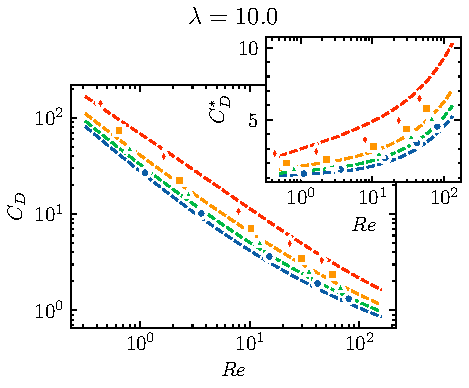
\includegraphics[height = 0.3\textwidth]{image/HOMOGENEOUS_final/CA/Cp_l_10.pdf}
    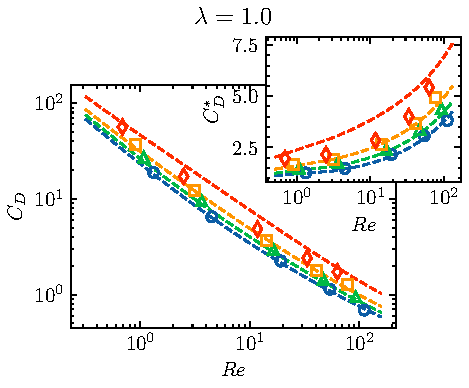
\includegraphics[height = 0.3\textwidth]{image/HOMOGENEOUS_final/CA/Cp_l_1.pdf}
    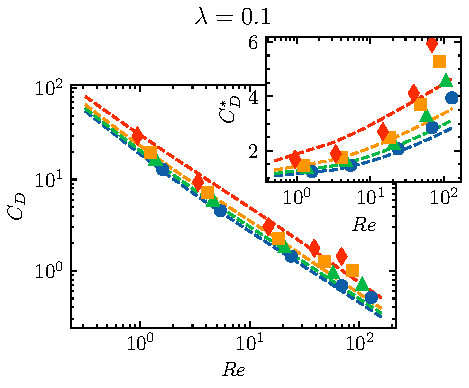
\includegraphics[height = 0.3\textwidth]{image/HOMOGENEOUS_final/CA/Cp_l_0.pdf}
    \caption{
        (main figures)
        Drag force coefficient in terms of the \textit{Reynolds} number. 
        (sub figures) Dimensionless drag force $C_d^* =C_d Re \frac{1}{8}\frac{\lambda+1}{3\lambda +2}$. 
        (symbols) DNS results for various values of $\phi$, 
        ($\pmb\bigcirc$) $\phi = 0.01$; ($\pmb\triangle$) $ \phi = 0.05$; ($\pmb\square$) $\phi = 0.1$ ($\pmb\lozenge$) $\phi = 0.2$.
        (dashed lines) Semi-empirical formula \ref{eq:C_d_finalRe}. 
        }
    \label{fig:cp}
\end{figure}

However, for $\lambda = 0.1$ the results are less satisfactory. 
In the dilute regime ($\phi = 0.01$) \ref{eq:CD0} does not accurately predict the drag coefficient (see \ref{fig:cp} (right)). 
This discrepancy might come from two factors: either \ref{eq:mei} fails to capture the drag force for isolated bubbles with a density ratio close to $1$  ($\zeta  = 0.9$).
Or the effect of the volume fraction is already significant, at these \textit{Reynolds} numbers, and is not properly accounted for by \ref{eq:geenralizedh} or \ref{eq:final_n}. 
Given that \ref{eq:mei} has been extensively validated in the literature for bubbles and that in the steady-state regime the density ratio is not supposed to impact the drag force term, we conclude that the second assumption is likely to be responsible for the inaccuracy. 
For $Re < 50$ and for all $\phi$ and $\lambda$,  \ref{eq:C_d_finalRe} perform very well. 


\subsection{Sedimentation velocity}



To ensure the consistency of our model, we now compare the \textit{Reynolds} numbers computed from our DNS with the theoretical predictions. 
To compute the mean relative velocity based on our new drag force model, we inject the expression of $C_D$ given by \ref{eq:C_d_finalRe}, into \ref{eq:C_d_adim}, and solve the equation for $Re$. 
As the resulting equation is not directly invertible, we use the iterative Newton-Raphson method to obtain the solutions, i.e. we solve for the $Re$ number in terms of $\phi$, $Ga$, and $\lambda$. 
Both, the theoretical prediction and the $Re$ measured in our DNS are divided by $Re_\text{stokes} = \frac{8}{Re} \frac{3\lambda +2}{\lambda+1}$ which represents the sedimentation \textit{Reynolds} number of an isolated particle in Stokes flow.  

The dimensionless sedimentation \textit{Reynolds} numbers are displayed in \ref{fig:Reasim}. 
\begin{figure}[h!]
    \centering
    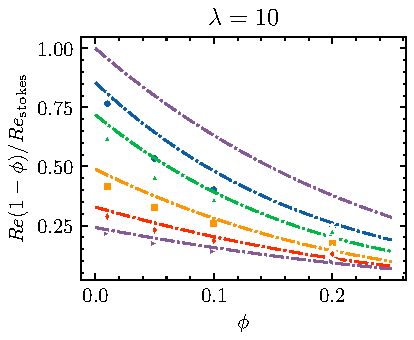
\includegraphics[height = 0.23\textwidth]{image/HOMOGENEOUS_final/CA/U_l_10.pdf}
    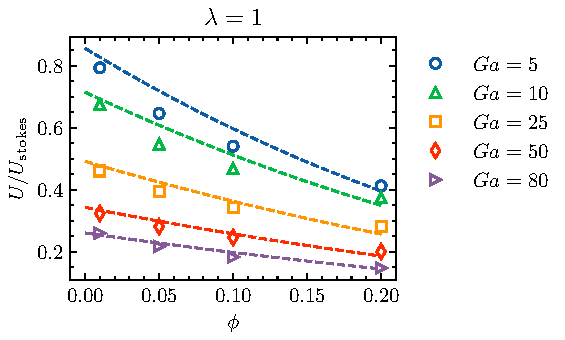
\includegraphics[height = 0.23\textwidth]{image/HOMOGENEOUS_final/CA/U_l_1.pdf}
    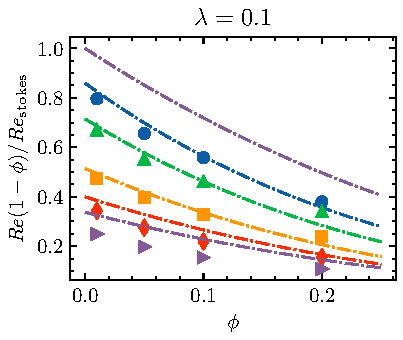
\includegraphics[height = 0.23\textwidth]{image/HOMOGENEOUS_final/CA/U_l_0.pdf}
    \caption{
        \textit{Reynolds} number based on the superficial velocity divided by the \textit{Reynolds} number of an isolated particle in stokes flow $Re_\text{stokes}= \frac{8}{Re} \frac{3\lambda +2}{\lambda+1}$, in terms of the volume fraction $\phi$, for various viscosity ratio, (left) $\lambda  = 10$ (middle) $\lambda =1$ and (right) $\lambda = 0.1$. 
        The symbols represent the different \textit{Galileo} numbers. 
        (dashed lines) Theoretical prediction form \ref{eq:CD0}. 
        (dot dashed lines) Theoretical prediction form \ref{eq:CD0} at $Re = 0$ corresponding to the simple relation \ref{eq:Richardson} with $n$ given by \ref{eq:n}. 
    }
    \label{fig:Reasim}
\end{figure}
The same observations as noted for the previous figure can be made regarding the accuracy of \ref{eq:C_d_finalRe} at $\lambda = 0.1$ for high $Re$. 
In these figures, we aim to address the validity of \ref{eq:geenralizedh}, and \ref{eq:final_n}. 
This requires verifying if the slope of the sedimentation velocity in terms of the volume fraction $\phi$ is well predicted by our semi-empirical model \eqref{eq:C_d_finalRe}. 

First, we focus on the low inertial cases ($Ga = 5$), to assess whether \ref{eq:geenralizedh} which is somewhat arbitrary for $Re \approx 1$ performs well. 
Specifically, by comparing \ref{fig:Reasim} (dot-dashed lines) and the case $Ga =5$ for $\lambda=0.1$ we observe that even at this low \textit{Galileo} number, the trends with the volume fraction already exhibit inertial effects. 
Indeed, our prediction at $Ga =5$ already exhibits large differences in slop with the Stokes prediction given by: $(1-\phi)^{n(Re=0)}$. 
At $\lambda = 0.1$ and $Ga = 5$ the Reynolds numbers obtained for these DNS are $Re = 1.10, 0.80, 0.64, 0.43$ for $\phi = 0.01, 0.05, 0.1, 0.2$, respectively.
Thus, this case lies exactly within the transitional zone introduced by \ref{eq:geenralizedh}. 
Thus, the good agreement of \ref{eq:C_d_finalRe} with the numerical data for $Ga = 5$ and $\lambda = 0.1$ serves as a validation for \ref{eq:geenralizedh}, since the latter formula seems to be representative in the transitional regime. 
For $\lambda = 1$ and $\lambda = 0.1$, with $Ga = 5$, we obtain $Re = 1.60 \to 0.68$ for $\phi = 0.01 \to 0.2$.
Thus, these cases are located in the transitional regime as well.  
Therefore, the good agreement of the DNS results for these cases with \ref{eq:C_d_finalRe} also confirms the good behavior of \ref{eq:geenralizedh}, and by extension, it also validates \ref{eq:final_n} for the low but finite $Re$. 


At high inertial effects ($Ga = 80$) we observe on \ref{fig:Reasim} (left) and (middle) that for $\lambda = 10$ and $1$, the slope of the theoretical prediction matches the DNS results. 
This means that the extension of \ref{eq:n_solid} for an arbitrary viscosity ration $\lambda$, i.e. the formula \ref{eq:n_final}, seems indeed validated at these \textit{Reynolds} numbers that ranges between $45$ and $128$ for these cases.  
However, at this stage, it is difficult to confirm the $2.4$ constant of \ref{eq:n_final} for arbitrary $\lambda$, as it would require reaching significantly higher ($Re > 500$) to enter this regime (see \ref{eq:n_jackson}). 

As previously noted for the drag force coefficient, when $\lambda=0.1$, slight discrepancies are observed between the DNS results and the predictions of \ref{eq:C_d_finalRe} for the sedimentation velocity at $Ga = 80$, (see \ref{fig:Reasim} (right)). 
Nevertheless, we can observe that the slope predicted by our model does not seem wrong compared to our DNS results. 
Instead, our model overpredicts the value of $Re (1-\phi)  / Re_\text{stokes}$  for  $Ga = 80$ in the dilute regime ($\phi = 0.01$), an error that carries over to the higher volume fractions. 
Note that the error in the rising velocity is bounded to $20\%$ for all cases, which is acceptable. 

In summary, \ref{eq:geenralizedh} and \ref{eq:final_n} for arbitrary $\lambda$ at $Re \ge 1$ seem to accurately represent the behavior observed in our numerical data. 
Since these two equations were the only unsupported assumptions in our entire reasoning, we can assert that \ref{eq:C_d_finalRe} remains physically consistent across the three-dimensional phase space defined by $\lambda$, $Re$, and $\phi$.
While minor improvements could be made to correct the results for the $\lambda = 0.1$ case at  $Re\approx 100$, we chose not to overfit on our dataset, maintaining a robust drag force model validated over a wide ranges of numerical and experimental measurements.